\chapter{Experimental Apparatus}\label{chap:experiment}

\section{Particle Accelerators}\label{sec:accelerators}

	To study the Standard Model, the Higgs boson, and hints of new physics, particle accelerators are used. Particle accelerators can be categorized as either fixed target or colliders. As the naming suggest, in a fixed target accelerator the beam hits a target that then produces the desired particle collisions. Whereas a collider uses two opposite circulating beams that are then brought to collide inside a detector. A fixed target accelerator energy scales as $E_{CM} = \sqrt{E_{beam}}$ whereas a collider scales as $E_{CM} = 2 \, E_{beam}$. 

	\subsection{Hadron Colliders}\label{ssec:hadron-colliders}

		There are two main types of particle colliders, those that use hadrons and those that use leptons. Lepton colliders are often referred to as precision machines, as the longitude momentum is known and backgrounds are well understood. The center of mass energy is well controlled in a lepton collider, meaning particles can be produced on resonance. On the other hand, due to the nature of hadrons not being fundamental particles a hadron collider produces a wide range of collisions. The constituents of a hadron participate in the collisions, meaning it is impossible to know the exact longitude momentum of the initial state. It is because of this exact reason that hadron colliders are referred to as discovery machines. The synchrotron radiation produced from a hadron collider is much lower than that of a lepton collider; meaning the beams are easier to control and can be pushed to higher energies without extra loses. The center of mass energy scales with $\frac{1}{m^4}$ in a hadron collider; again leading to an increased energy gain by simply using heavier particles.

	\subsection{The Large Hadron Collider}\label{ssec:LHC}

		The Large Hadron Collider (LHC) is a 27 km circumference circular collider built outside of Geneva, Switzerland at CERN (Conseil Européen pour la Recherche Nucléaire). At center of mass energy $13.6$ TeV, the LHC is the largest and highest energy particle accelerator ever built. There are four main collision points along the LHC: the ATLAS, CMS, ALICE, and LHCb experiments. ATLAS and CMS are general purpose particle detectors while ALICE and LHCb focus on heavy ion collisions. The numbers stated in the following sections are in reference to proton-proton collisions.

		The LHC consists of 1104 NbTi superconducting dipole magnets, each being 15 m long, weighing 35 tonnes, cooled to 2 K, operating at 11,000 Amps, and produce a magnetic field of 8.3 T. A cross-section of a dipole magnet and the surrounding cryogenic system can be see in figure \ref{fig:dipole-xsec}. The dipole magnets are used to bend the beam around the ring with another 128 used in the beam dump system to remove the beam safely from the LHC. A 2-in-1 configuration is used within the dipole magnets to create the required magnetic fields to bend two equally charged beams in opposite directions. A diagram of the magnetic fields in this configuration produced can be seen in \ref{fig:dipole-field}. To focus the beam in the horizontal and vertical planes two quadrapole magnets are used; one magnet focuses in one plane while defocusing in the other. The end result is a horizontally and vertically focused beam. While in the LHC, the hadrons are accelerated using radiofrequency cavities. Table \ref{tab:LHC} lists some information on the LHC. 

		\begin{table}[!thp]
			\centering
			\caption{LHC parameters  \cite{lhc-facts}}
			\begin{tabular}{| l | l |}  
			\hline
			Circumference 						& $26,659$ m 					\\ 	\hline
			Dipole operating temperature 		& $1.9$ K 						\\ 	\hline
			Dipole magnets 						& $1232$ 						\\	\hline
			Quadrapole magnets 					& $392$ 						\\	\hline
			Radiofrequency cavities 			& $16$ ($8$ per beam) 			\\ 	\hline
			Beam energy 						& $6.5$ TeV ($13$ CoM TeV) 		\\ \hline
			Protons per bunch 					& $1.2 \mathrm{x} 10^11$ 		\\ \hline
			Bunches per beam 					& $2808$ 						\\ \hline
			Revolutions per second 				& $11245$ 						\\ \hline
			Collisions per second 				& $1,000,000,000$ 				\\ \hline
			\end{tabular}
			\label{tab:LHC}
		\end{table}

		\begin{figure}[!ht]
		\centering
		\includegraphics[width=\textwidth,keepaspectratio=true]{chapters/chapter3_experiment/images/dipole-crosssection.png}
		\caption{Cross-section of cryodipole (lengths in mm). \cite{lhc-machine}}
		\label{fig:dipole-xsec}
		\end{figure}

		\begin{figure}[!ht]
		\centering
		\includegraphics[width=.45\textwidth,keepaspectratio=true]{chapters/chapter3_experiment/images/dipole-field.jpeg}
		\caption{Field of the LHC dipole magnets. \cite{dipole-field}}
		\label{fig:dipole-field}
		\end{figure}

	\subsection{CERN Accelerator Complex}\label{ssec:cern-accelerators}
		There are a series of accelerators used to get each beam up to its final energy of 6.5 TeV. The protons used in collisions are sourced from hydrogen atoms. The hydrogen is ionized, leaving the nucleus consisting of one proton, these protons are then accelerated in radiofrequency (RF) cavities. Figure \ref{fig:CERN-complex} shows in detail the full accelerator complex at CERN.\footnote{Figure \ref{fig:CERN-complex} shows the newer LINAC 4 at the start of Run-3. This work is concerning data taken with LINAC 2.} 
		\begin{figure}[!ht]
		\centering
		\includegraphics[width=\textwidth,keepaspectratio=true]{chapters/chapter3_experiment/images/CERN-complex.png}
		\caption{The CERN accelerator complex. \cite{CERN-complex}}
		\label{fig:CERN-complex}
		\end{figure}
		The protons used in the LHC start the accelerating process in the linear accelerator LINAC 2. They then are accelerated in the booster, PS, SPS, and are finally injected at the LHC where they are accelerated to the final 6.5 TeV beam energy. The final energies of protons from each accelerator can be seen in Table \ref{tab:accelerator-complex}.
		\begin{table}[!thp]
			\centering
			\caption{Accelerator final energies}
			\begin{tabular}{| l | l |}  
			\hline
			Accelerator 					& Final Energy 	\\ \hline
			\hline
			LINAC 2 						& $50$ MeV 		\\ 	\hline
			Booster 						& $1.4$ GeV 	\\ 	\hline
			Proton Synchrotron (PS)			& $26$ GeV 		\\ 	\hline
			Super Proton Synchrotron (SPS) 	& $450$ GeV 	\\ 	\hline
			Large Hadron Collider (LHC)		& $6.5$ TeV 	\\ 	\hline
			\end{tabular}
			\label{tab:accelerator-complex}
		\end{table}

	\subsection{Luminosity}\label{ssec:lumi}
		The amount of data collected from colliders is often referred to in terms of luminosity. Luminosity is measured in terms of inverse barns, where $1 \, b = 10^{-28} \, m^2$. Instantaneous luminosity of one bunch crossing can be written as 
		\begin{equation}\label{eqn:bunch-lumi}
		\mathcal{L}_{bunch} = \frac{ \mu  f }{\sigma}
		\end{equation}
		where $\sigma$ is the cross section and can be thought of as the probability of a collision occurring, $\mu$ is the number of inelastic interactions per bunch crossing, and $f$ is the revolution frequency of the LHC $f=11246$ Hz. Therefore, the total instantaneous luminosity is 
		\begin{equation}\label{eqn:tot-inst-lumi}
		\mathcal{L} = N_b \frac{ \langle \mu \rangle f}{\sigma}
		\end{equation}
		where $\langle \mu \rangle$ is the average number of inelastic interactions per bunch crossing. 

		The integrated luminosity then corresponds to the total amount of data that was taken during a time period and can be seen for the LHC Run-2 in \ref{fig:lhc-lumi}
		\begin{figure}[!ht]
		\centering
		\includegraphics[width=.65\textwidth,keepaspectratio=true]{chapters/chapter3_experiment/images/intlumivstimeRun2DQall.png}
		\caption{ Cumulative luminosity versus time delivered to ATLAS (green), recorded by ATLAS (yellow), and certified to be good quality data (blue) during stable beams for pp collisions at 13 TeV center of mass energy in 2015-2018. The difference between the colored histograms reflects inefficiencies, especially those seen when restarting data taking. }
		\label{fig:lhc-lumi}
		\end{figure}
		The value of $\langle \mu \rangle$ changed throughout data taking and can be seen in Figure \ref{fig:run2-mu} and is referred to as pileup because the higher the $\langle \mu \rangle$ value, the more messy a collision becomes.
		\begin{figure}[!ht]
		\centering
		\includegraphics[width=.65\textwidth,keepaspectratio=true]{chapters/chapter3_experiment/images/mu_2015_2018.png}
		\caption{ The luminosity-weighted distribution of the mean number of interactions per bunch crossing for the 2015-2018 \pp collision dataset at $13$ TeV center of mass energy. }
		\label{fig:run2-mu}
		\end{figure}
		The effect of high pileup can be seen in Figure \ref{fig:high-pileup-event-display}, a collision event taken in 2018 with 29 reconstructed vertices shown on the bottom right as colored circles.
		\begin{figure}[!ht]
		\centering
		\includegraphics[width=\textwidth,keepaspectratio=true]{chapters/chapter3_experiment/images/event_display_r349114_e216445472_v4_wMoreTracks_v3_wAtlantisTrackColor_Inset.png}
		\caption{ A display of a candidate Z boson event from proton-proton collisions recorded by ATLAS with LHC stable beams at a collision energy of 13 TeV. The Z boson candidate is reconstructed in a beam crossing with 28 additionally reconstructed primary vertices from the minimum bias interactions. The candidate event is reconstructed in the 2$\mu$ final state. In the left display, the red lines show the path of the two muons including the hits in the muon spectrometer and the yellow tracks are the remaining charged particles from the 29 vertices, with transverse momentum above 0.5 GeV. The colored squares in the lower display correspond to the position of the reconstructed vertices. The invariant mass of the two muons is 92.3 GeV. }
		\label{fig:high-pileup-event-display}
		\end{figure}


		A common calculation using the total integrated luminosity is shown in Equation \ref{eqn:tot-proc-num}; where the number of times a particular process was produced is calculated.
		\begin{equation}\label{eqn:tot-proc-num}
		N_{x} = \mathcal{L} \sigma_{x}
		\end{equation}
		where again, $\sigma$ is the cross section. In this case, the cross section corresponding to process $x$.


\section{The ATLAS Detector}\label{sec:ATLAS}
	The ATLAS (\textbf{A} \textbf{T}oroidal LHC \textbf{A}pparatu\textbf{S}) detector is one of two general purpose particle detectors on the LHC. The other being the \textbf{C}ompact \textbf{M}uon \textbf{S}olenoid (CMS). ATLAS, like other particle detectors, is comprised of four main components; the inner detector, calorimeters, muon system, and the magnet system. Each component has several types of technology in order to measure the energy of all possible particle decays.\footnote{Neutrinos are not directly detected, but inferred via a missing transverse energy calculation described in Section \ref{sec:reco-etmiss}.} The full ATLAS detector measures 44 m in length, 25 m in diameter, and weighs over 7000 tonnes. Figure \ref{fig:ATLAS} shows a 3D model of the ATLAS detector and Figure \ref{fig:ATLAS-XSec} shows a cross section of the detector and various particles trajectory.\footnote{Figure \ref{fig:ATLAS} shows the New Small Wheel muon-chambers. This dissertation concerns data collected with the old Small Wheel muon-chambers.} All of the subdetectors output data to the Trigger and Data Acquisition (TDAQ) system that selects collisions with interesting physics using a complex mix of hardware and software algorithms detailed in \ref{ssec:trigger}. 

	\begin{figure}[!ht]
	\centering
	\includegraphics[width=.75\textwidth,keepaspectratio=true]{chapters/chapter3_experiment/images/ATLAS_3d_run3.png}
	\caption{ Cut-away view of the ATLAS detector with major subdetectors highlighted.}
	\label{fig:ATLAS}
	\end{figure}

	\begin{figure}[!ht]
	\centering
	\includegraphics[width=.65\textwidth,keepaspectratio=true]{chapters/chapter3_experiment/images/ATLASCrossSectionDiagram.png}
	\caption{ Cross section view of the ATLAS detector with subdetectors labeled. Various types of particles radial trajectories are shown.}
	\label{fig:ATLAS-XSec}
	\end{figure}

	\subsection{Detector Coordinates}\label{ssec:coordinates}
	Since ATLAS is a cylinder, it is convenient to start with polar cylindrical coordinates. For ATLAS, the z-axis is inline with the beam line, the x-axis points towards the center of the LHC ring, and the y-axis points vertically. However, since particle collisions are relativistic by nature, a set of Lorentz invariant coordinates is much more useful. The radial coordinate r defines the radial distance from the interaction point (IP) at the center of ATLAS, $\phi$ is the azimuthal angle describing the angle from the x-axis in, and $\eta$, the pseudorapidity, is defined as 
	\begin{equation}\label{eqn:eta}
	\eta \equiv - ln(tan(\frac{\theta}{2}))
	\end{equation}
	where $\theta$ is the angle from the y-axis. It is in the differences in $\eta$ between particles that provides the Lorentz invariance in this coordinate system of $(r,\phi,\eta)$. Due to the large collision energies of the LHC, the pseudorapidity is a close estimate to the true rapidity of the particles. 
	\begin{equation}\label{eqn:rapidity}
	y \equiv \frac{1}{2} ln(\frac{E+p_Z}{E-p_Z}) \approx \eta
	\end{equation}
	When speaking of differences in particle locations within ATLAS, $\Delta R$  is often used.
	\begin{equation}\label{eqn:dR}
	\Delta R \equiv \sqrt{ (\Delta \eta)^2 + (\Delta \phi)^2}
	\end{equation}

	% In the ATLAS detector, the central barrel section corresponds to $|\eta| < 2.5$
	Figure \ref{fig:pseudorapidity} shows visually how $\eta$ relates to $\theta$. In the ATLAS detector, the central barrel section corresponds to a range of $|\eta|<1$. 

	\begin{figure}[!ht]
	\centering
	\includegraphics[width=.25\textwidth,keepaspectratio=true]{chapters/chapter3_experiment/images/Pseudorapidity.png}
	\caption{ A diagram showing the pseudorapidity $\eta$ and corresponding $\theta$ values. \cite{pseudorapidity} }
	\label{fig:pseudorapidity}
	\end{figure}

	\subsection{Magnet Systems}\label{ssec:magnets}
	The ATLAS detector makes use of two superconducting magnet systems; a central solenoid and a toroid system. Both systems provide large magnetic fields to curve charged particles. The curvature can be used to measure the electromagnetic charge and charge to mass ratio, effectively measuring the momentum of charged particles. Figure \ref{fig:ATLAS-magnets} shows the magnets in ATLAS.

	\begin{figure}[!ht]
	\centering
	\includegraphics[width=.65\textwidth,keepaspectratio=true]{chapters/chapter3_experiment/images/magnetSystems.png}
	\caption{ The ATLAS magnet systems.}
	\label{fig:ATLAS-magnets}
	\end{figure}

	\subsubsection{Solenoid System}\label{sssec:solenoid}
	The central solenoid encases the Inner Detector (ID), creating an axially symmetric 2 T magnetic field. This magnetic field bends charged particles in the transverse plane throughout the ID. The solenoid magnet itself measures 5.3 m in length and 2.63 m in diameter. In an effort to decrease the amount of material in front of the calorimeters the solenoid magnet was made to be thin. It is a single-layer coil with approximately 1200 turns of NbTi superconducting wires encased in Al-Cu to structurally stabilize the magnet material \cite{atlas-solenoid}. The steel structure within the Tile calorimeter acts as the magnetic flux return for the solenoid magnet system. 70\% of this flux passes through the supporting girder structure, 25\% through the active calorimeter material, and roughly 2\% through the front-plates of the Tile calorimeter \cite{ATLAS-tile}.

	\subsubsection{Toroid System}\label{sssec:toroid}
	The ATLAS detector gets its name from the toroid magnetic system that is critical in the identification of high energy muons. The toroid system bends any charged particles that make it past the calorimeters along the beam axis. This is achieved through a radially symmetric magnetic field of 3.9 T in the barrel and 4.1 in the end-caps. The barrel toroid system is comprised of 8 air core superconducting toroid magnets that each measure 25 m in length, 10 m in diameter, and weigh 750 tonnes. The superconducting wires are the same used in the solenoid, NbTi encased in Al-Cu \cite{atlas-toroid}. Each magnet is encased in a stainless steel cryogenic chamber, or cryostat. The toroid magnet system has two end-cap toroids that are very similar in construction to the barrel toroids. The end-cap toroids also have 8 coils measuring 5 m in length and 10 m in diameter. Instead of individual cryostats for each coil, the end-caps are encased in large cryostats that hold all 8 coils. This allows the end-caps to be pulled out and offers easy access to the rest of the detector. Just like with the central solenoid system, the design of the toroid system was chosen to limit the amount of material between detector components. A solenoid magnet of similar size to the toroid system would not only add more material, but would be cost prohibitive as well.


	\subsection{Inner Detector}\label{ssec:ID}
		\begin{figure}[!ht]
		\centering
		\subfloat[\label{fig:hpm-diagrams_a}]{\includegraphics[width=.55\textwidth,keepaspectratio=true]{chapters/chapter3_experiment/images/ATLAS_ID_Run3.png}}
		\subfloat[\label{fig:hpm-diagrams_b}]{\includegraphics[width=.45\textwidth,keepaspectratio=true]{chapters/chapter3_experiment/images/ATLAS_ID_Transverse_View.png}}
		\caption{\label{fig:ATLAS-ID} (a) Cut-away view of the ATLAS Inner Detector. (b) Cross-sectional view of the ATLAS Inner Detector.}
		\end{figure}

		The ID is the inner-most detector, closest to the IP and is used to track the trajectory of charged particles leading to the measurement of electromagnetic charge and momentum. The ID is immersed in the 2 T magnetic field provided by the central solenoid described in section \ref{sssec:solenoid} and covers a pseudorapidity range of $|\eta|<2.5$. The three subdetectors within the ID can be seen in Figure \ref{fig:ATLAS-ID}, the Pixel, \textbf{S}emi\textbf{C}onductor \textbf{T}racker (SCT), and the \textbf{T}ransition \textbf{R}adiation \textbf{T}racker (TRT). Like the toroid system, and many of the other subdetectors, the ID is comprised of barrel and end-cap segments. The ID barrel section is 1.6 m in length and covers $|\eta|<1$ while the end-caps measure over 7 m in length and cover $1 < |\eta| < 2.5$. 

		A track is considered good if there are hits in at least 3 pixel layers and 8 strips. The ID tracking system was designed with a resolution of 
		\begin{equation}\label{eqn:tracking-resolution}
		\frac{\sigma_{\pt}}{\pt} = 0.05 \% \, \pt \oplus 1\%
		\end{equation}
	
		\subsubsection{Pixel}\label{sssec:pixel}
		The detector closest to the beam and IP is the Pixel Detector. The Pixel Detector is designed to measure with high-precision and high-granularity. The barrel Pixel detector consists of three layers of n-type silicon substrate with n-type implants. The closest layer to the IP sits at 50.5 mm and the outermost layer extends out to 12 cm. This combination gives the Pixel Detector the ability to determine the impact parameters of collisions with incredible precision. Due to the high radiation dose this close to the IP, the Pixel Detector was designed to be operated only in partial depletion. Each pixel cell measures $200 \mu m \times 400 \mu m \times 250 \mu m$. There are five Pixel disks on each end-cap of the ID. In total there are 1,744 modules, 46,080 readout channels per module, giving over 80 million channels with a spatial resolution of $10 \, \mu m (R-\phi) \times 115 \, \mu m (z)$ \cite{ATLAS-pixel}. 

		In order to keep up with the increased demand of Run-2 data taking conditions, an additional layer of pixels was installed in the Long Shutdown 1 (LS1) between 2013 and 2015. This \textbf{I}nsertable \textbf{B} \textbf{L}ayer (IBL) provides even finer granularity tracking with pixel cells measuring $50 \, \mu m \times 250 \, \mu m$ installed at a radial distance of $R=33.25$ mm from the IP and a spatial resolution of $8 \, \mu m (R-\phi) \times 40 \, \mu m (z)$ \cite{ATLAS-IBL}. The IBL has proved incredibly useful in the reconstruction of displaced vertices from processes like \bjet hadronization and $\gamma \rightarrow e^+ e^-$.

		\subsubsection{Semiconductor Tracker}\label{sssec:SCT}
		Moving radially outward, the next subdetector is the SCT that provides tracking in the intermediate radial range from the IP and covers a range of $|\eta| < 2.5$. Similar to the Pixel Detector, the SCT has 4 barrel layers and 9 end-cap wheels on each side. The SCT provides four measurements per track via silicon microstrip detectors. Each microstrip is made of two $6.36 \times 6.40 \, cm^2$ detectors glued end to end so each microstrip is $12.8 \, cm$ long. Two microstrips are then glued back to back with a $40 \, \mu rad$ angle. In total there are 768 strips, giving 6.2 million readout channels. The SCT has a spatial resolution of $17 \, \mu m (R-\phi) \times 580 \,\mu m (z)$ and can distinguish tracks with as small as a $200 \, \mu m$ separation \cite{ATLAS-ID}.

		\subsubsection{Transition Radiation Tracker}\label{sssec:TRT}
		The final subdetector of the ID is the TRT $(R=554 \, \mathrm{mm} \, - 1082 \, \mathrm{mm})$ . Instead of silicon detectors the TRT uses 4 mm diameter straw tubes; a hollow tube with a sense wire held at high voltage in the middle. The max length of a straw is 150 cm. The straws are filled with a gaseous mixture of $70\% \, \mathrm{Xe,} \, 27\% \, \mathrm{CO}_2, \, 3\% \, \mathrm{O}_2$.\footnote{During Run-2 the Xe was replaced with Ar as a cost saving measure. Ar provides similar performance as Xe in tracking, but is less efficient in absorbing X-rays from transition radiation.} Charged particles ionize the gas mixture, thereby releasing an electron and an ion. The ion drifts to the straw surface and the electron drifts to the wire; this charge drift is then measured as a signal. The TRT checks the signals against two thresholds, a lower threshold for measuring the drift time to derive a position and a higher threshold that is used to identify transition radiation X-rays. The higher threshold provides discriminating power between charged pions and electrons.

		The TRT consists of a barrel section and 18 wheels in each end-cap. In the barrel, there are 50,000 straws divided in two at the center to allow for two separate readouts. The end-caps have 320,000 straws. In total, there are 420,000 readout channels. Each straw provides a spatial resolution of $170 \mu m$. \cite{ATLAS-ID}

	\subsection{Calorimeters}\label{ssec:calorimeters}
	The ATLAS detector makes use of two types of sampling calorimeters, one that uses liquid argon as the active medium and another that uses scintillating plastic tiles. Both types of calorimeters are designed to fully absorb particles via showering. Incoming particles interact with an absorber material and generate secondary particles. Those secondary particles interact with the absorber and create another set of particles. This cascading effect creates showers of particles inside the calorimeters. The shape and depth of these particles is important in the design choices for the calorimeters as well as particle identification. Two helpful variables when talking about shower depth are radiation length $\chi_0$ and nuclear interaction length $\lambda$. $\chi_0$ is defined as the distance where a particle has lost energy via bremsstrahlung equal to $\frac{1}{e}$.\footnote{$\chi_0$ can also be defined as $\frac{7}{9}$ of the mean free path of a high energy photon.} Whereas $\lambda$ is the mean free path of a hadron before undergoing a inelastic nuclear interaction. In order to fully absorb a wide energy range of incident particles the calorimeters are such that any path through them is at least $25 \, \chi_0$ or $10 \, \lambda$. Figure \ref{fig:calo-interaction-length} shows the calorimeters and their nuclear interaction lengths as a function of $\eta$.

	\begin{figure}[!ht]
	\centering
	\includegraphics[width=.65\textwidth,keepaspectratio=true]{chapters/chapter3_experiment/images/Calo_Interaction_Lengths.png}
	\caption{ Interaction lengths as a function of $\eta$ in the ATLAS calorimeters. The unlabeled brown color is the material in front of the EM calorimeters and the unlabeled cyan is the amount of material in front of the first active layer of the muon spectrometer. \cite{atlas-experiment}}
	\label{fig:calo-interaction-length}
	\end{figure}

	The design resolution of the calorimeters can be seen in Table \ref{tab:calo-resolution}.

	\begin{table}[!thp]
	\centering
	\caption{ Design resolution of EM and hadronic calorimeters in the ATLAS Detector.}
	\resizebox{.45\textwidth}{!}{\begin{tabular}{| c | c | c |}  
	\hline
	Calorimeter											& Pseudorapidity range 																		& Resolution \\[1ex] \hline 
	Electromagnetic 									& $| \eta | < 3.2$ 																			& $\frac{\sigma}{E} = \frac{10\%}{\sqrt{E}} \oplus 0.7\%$ \\[1ex] \hline
	\multicolumn{1}{|c|}{\multirow{2}{*}{Hadronic}} 	& \begin{tabular}[c]{@{}c@{}} $| \eta | < 3.2$ \\[1ex] $3.1 < | \eta | < 4.9$ \end{tabular} & \begin{tabular}[c]{@{}c@{}} $\frac{\sigma}{E} = \frac{50\%}{\sqrt{E}} \oplus 3\%$ \\[1ex] $\frac{\sigma}{E} = \frac{100\%}{\sqrt{E}} \oplus 10\%$ \end{tabular} \\ \hline 
	\end{tabular}}
	\label{tab:calo-resolution}
	\end{table}

	The layout of calorimeters in the ATLAS detector can be seen in Figure \ref{fig:calo-layout}.
	\begin{figure}[!ht]
	\centering
	\includegraphics[width=.85\textwidth,keepaspectratio=true]{chapters/chapter3_experiment/images/ATLAS_Calorimeters_Run3.png}
	\caption{ Cut-out view of the ATLAS detector's calorimeters.}
	\label{fig:calo-layout}
	\end{figure}

		\subsubsection{Liquid Argon Calorimeters}\label{sssec:LAr}
		A liquid argon (LAr) is based on a similar principle to the straw tubes of the TRT described in section \ref{sssec:TRT}. In this case, the LAr is the active medium that is ionized by the incoming particle. The free electron then drifts to an electrode, copper-tungsten in the case of the barrel LAr calorimeter. The drifting electrons are then readout as an electrical signal; there are approximately 180,000 LAr readout channels in the ATLAS detector. LAr was chosen as the active medium due to it's intrinsic radiation hardness, stability over time, and linear response. The LAr must be kept at very cold temperatures, around 85 K. To achieve this, the LAr calorimeters are kept in cryostats, the barrel calorimeter shares the cryostat and vacuum with the central solenoid.

		There are four LAr calorimeters within the ATLAS detector. The main barrel section (EMB) is designed for electromagnetic calorimetry with a lead-stainless steel absorber and covers a pseudorapidity range of $|\eta|<2.5$. Next in $\eta$ is the LAr Electromagnetic End-Cap (EMEC) that also uses lead-stainless steel absorber and the LAr Hadronic End-Cap (HEC) which has a copper plate absorber; both EMEC and HEC cover $1.5 < |\eta| < 3.2$. The final LAr calorimeter is the aptly named Forward Calorimeter (FCAL) that covers $|\eta|<4.9$ and has three modules. The first is optimized for EM calorimetry and uses a copper absorber. The other two FCAL modules are used to measure hadronic showers and use tungsten absorbers.

		The EMB and EMEC both utilize an accordion geometry pictured in Figure \ref{fig:LAr-accordion} to ensure a full $\phi$ coverage. 
		\begin{figure}[!ht]
		\centering
		\includegraphics[width=.45\textwidth,keepaspectratio=true]{chapters/chapter3_experiment/images/LAr_Accordion_Geometry.png}
		\caption{ A EMB module showing the accordion geometry and granularity. \cite{atlas-experiment}}
		\label{fig:LAr-accordion}
		\end{figure}
		The EMB consists of four layers, the first being a LAr presampler of 1.1 cm thickness. The presampler is used to correct for energy losses due to material in front of the calorimeter. The first layer after the presampler is finely segmented to ensure good position measurements. The second layer is $16 \, \chi_0$ thick and collects most of the electromagnetic showers. Typically, only the tails of EM showers make it to the third and final layer, so a courser granularity is used. 

		\subsubsection{Tile Calorimeter}\label{sssec:Tile}
		\begin{figure}[!ht]
		\centering
		\subfloat[\label{fig:tile-modules_a}]{\includegraphics[width=.45\textwidth,keepaspectratio=true]{chapters/chapter3_experiment/images/TileModuleCrossSection.png}} \\
		\subfloat[\label{fig:tile-modules_b}]{\includegraphics[width=.45\textwidth,keepaspectratio=true]{chapters/chapter3_experiment/images/Tile_Modules_Azimuth_View.png}}
		\caption{\label{fig:tile-modules} (a) Diagram of an individual TileCal module. (b) Azimuthal view of two TileCal modules with the IP being to the right.}
		\end{figure}
		The hadronic Tile Calorimeter (TileCal) is a sampling calorimeter that is designed to fully absorb hadronic showers covering a range of $|\eta|<1.7$ at a radial distance of $2.28 \, \mathrm{m} \leq R \leq 4.25 \, \mathrm{m}$ from the IP. This radial distance translates to approximately $7.4\, \lambda$. A similar design of absorber and electrode is used in TileCal to capture the full energy of hadronic showers. TileCal uses a steel absorber. However, instead of a liquid or gas being ionized and the free electrons being collected as a signal, TileCal takes advantage of a special material called scintillating plastic. When an ionizing particle interacts with the scintillating plastic, light is created; this light is absorbed in wavelength shifting (WLS) fibers. It is then re-emitted and transmitted to photomultiplier tubes (PMTs). The PMT signal is then shaped, amplified at two gains with a ratio of 64:1, then digitized at 40 MHz with 10-bit analogue-to-digital converters (ADCs). Each cell within TileCal has 2 PMTs, giving over 10,000 readout channels. There are 256 modules within TileCal. A diagram of an individual module and the layout of two modules side-by-side can be seen in Figure \ref{fig:tile-modules}.
		

		A significant fraction of the author's time and effort during their PhD went to data quality monitoring and maintenance of TileCal. These works are detailed in Appendix \ref{app:Tile-DQ}.

	\subsection{Muon Spectrometer}\label{ssec:muon-system}
	High momentum muons provide a vital signature at the LHC. Muons are minimally ionizing particles, meaning they leave a small amount of energy inside detectors and travel to the edge and beyond the volume of the ATLAS detector. Instead of attempting to fully absorb muons, high precision position measurements are taken to track their trajectories. The toroid magnet system described in section \ref{sssec:toroid} is an integral part of the Muon Spectrometer; it provides the bending force, changing the trajectories to the direction of the beamline. The barrel section of the Muon Spectrometer consists of three concentric cylindrical shells at $R=5 \, \mathrm{ m, }\, 7.5 \, \mathrm{ m, } \,  10 \, \mathrm{ m}$ made of Monitored Drift Tubes (MDTs) $(|\eta|<1)$. \cite{ATLAS-muon} These cylindrical shells sit in-between and on the air core toroid magnets. On the $2^{\mathrm{nd}}$ and $3^{\mathrm{rd}}$ shells are Resistive Plate Chambers (RPCs) that provide quick triggering. Complimenting the barrel section are the end-caps, referred to as wheels for the Muon Spectrometer. The wheels are placed at $|z|\approx 7.4 \, \mathrm{ m, } \, 10.8 \, \mathrm{ m, } \, 14 \, \mathrm{ m, and} \,21.5 \,\mathrm{ m }$ $(2.0 < |\eta| < 2.7)$. The innermost layer of these wheels experience the highest rates of incident particles. To cope with this, Cathode Strip Chambers (CSCs) with a finer granularity than the MDTs that are used in the barrel. Similarly, Thin Gap Chambers (TGCs) are used for triggering instead of RPCs. These wheels provide spatial coordinates orthogonal to those of the precision-tracking MDTs in the barrel. Figure \ref{fig:muon-spec} shows the positioning of the various Muon Spectrometer components.\footnote{Figure \ref{fig:muon-spec} Shows the New Small Wheel (NSW). The NSW is an upgrade to the old Small Wheels that were used in the data taking period that concerns this dissertation.}

	% \begin{figure}[!h]
	% \centering
	% \subfloat[\label{fig:muon-spec_a}]{\includegraphics[width=.45\textwidth,keepaspectratio=true]{chapters/chapter3_experiment/images/ATLAS_Muon_System_Run3.png}}
	% \subfloat[\label{fig:muon-spec_b}]{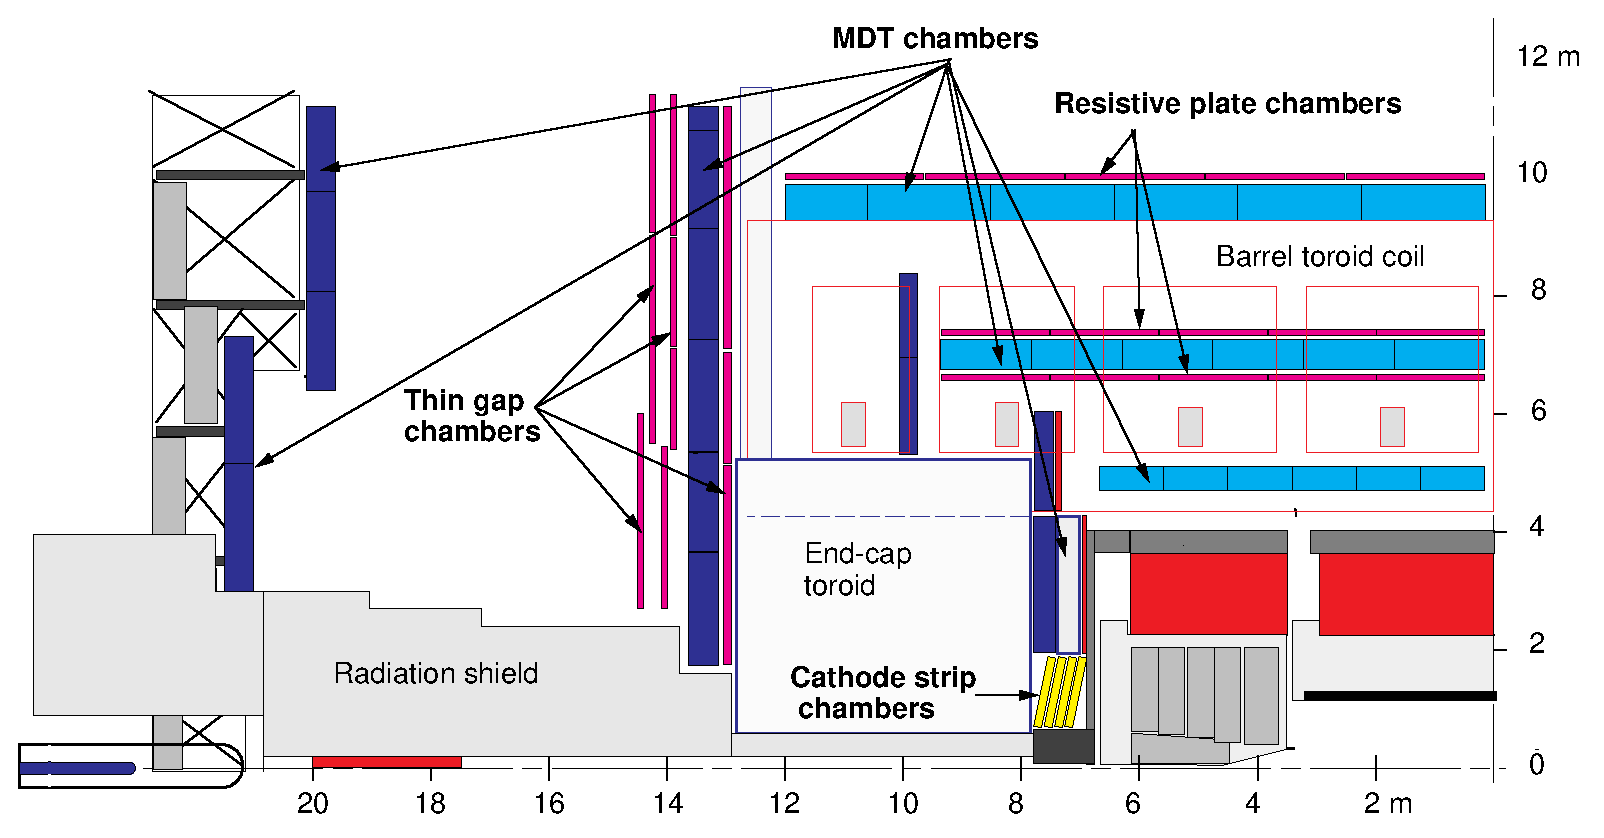
\includegraphics[width=.45\textwidth,keepaspectratio=true]{chapters/chapter3_experiment/images/ATLAS-muon-rz-tdr.eps}} \\
	% \subfloat[\label{fig:muon-spec_c}]{\includegraphics[width=.45\textwidth,keepaspectratio=true]{chapters/chapter3_experiment/images/ATLAS-muon-xy-tdr.eps}}
	% \caption{\label{fig:muon-spec} (a)   (b)}
	% \end{figure}

	\begin{figure}[!ht]
	\centering
	\includegraphics[width=\textwidth,keepaspectratio=true]{chapters/chapter3_experiment/images/ATLAS_Muon_System_Run3.png}
	\caption{Cut-out view of the ATLAS detector Muon Spectrometer.}
	\label{fig:muon-spec}
	\end{figure}

	\subsection{Trigger System}\label{ssec:trigger}
	The high luminosity provided by the LHC is critical in collecting enough data to make detailed physics analyses. However, it also means that there is an incredibly large amount of data to sort through. So much that it is not possible to write out the data from every bunch crossing. As shown in Figure \ref{fig:high-pileup-event-display}, even one single event can contain an inordinate amount of data. Another issue arises due to the nature of hadron collisions; in that not all bunch crossing provide hard scatter inelastic collisions that are ``interesting'' enough to save data on. 

	To solve this issue, the data coming out of ATLAS is combed through in real time at a variable rate of 1 kHz to 40 MHz. This is done with a Trigger and Data Acquisition (TDAQ) system. The TDAQ system used in Run-2 is described in detail here: \cite{ATLAS-trigger-Run2}. The TDAQ system reads in data from the ATLAS detector, calculates relevant quantities, and makes a decision on if there was an event worth storing. A diagram showing the data flow into the TDAQ system is show in \ref{fig:trigger-run2}.\footnote{Figure \ref{fig:trigger-run2} shows the Fast TracKer (FTK). During Run 2 FTK was undergoing commissioning and was not used in the active TDAQ system.} 
	\begin{figure}[!ht]
	\centering
	\includegraphics[width=\textwidth,keepaspectratio=true]{chapters/chapter3_experiment/images/Trigger_Run2.png}
	\caption{The ATLAS TDAQ system in Run-2 showing the components relevant for triggering as well as the detector read-out and data flow.}
	\label{fig:trigger-run2}
	\end{figure}
	The ATLAS TDAQ system consists of two main components, Level-1 (L1) and High Level Trigger (HLT). The L1 trigger is a hardware based trigger system that reads in data from the calorimeters and muon spectrometer. The L1 trigger has a latency of $2.5 \, \mu \mathrm{s}$ and can read-out accepted events up to 100 kHz, the detector maximum readout rate. The HLT is a software based trigger system based on the offline reconstruction software. During Run-2 the HLT operated with an average output rate of 1.2 kHz, which translates to about 1.2 GB/s of data sent to permanent storage.	

	After the TDAQ system accepts an event, the data is set to be stored on magnetic tape for long term storage. It is also processed at the local computing farm named Tier-0 with the full reconstruction software suite described in Chapter \ref{chap:reco}.

